\documentclass[a4paper]{article}

\usepackage[T1]{fontenc}
\usepackage[utf8]{inputenc}
\usepackage{gensymb}
\usepackage{pgfplots}
\usepackage{amsmath}
\usepackage{comment}
\usepackage[percent]{overpic}
\usepackage{makecell}
\usepackage{float}
\usepackage{wrapfig}
\usepackage{icomma}
\usepackage{subcaption}
\usepackage{diagbox}
\usepackage{tikz}

% Content of table can have multiple rows
\usepackage{multirow}

% Easily use 1st, 2nd, 3rd etc. in text
\usepackage[super]{nth}

% Indents from sides of paper, etc.
\usepackage[letterpaper]{geometry}
\geometry{verbose,tmargin=1.5cm,bmargin=2cm,lmargin=2cm,rmargin=2cm}

% Graphics operations
\usepackage{graphicx}

% Automatically indent the 1st paragraph in every section
\usepackage{indentfirst}

%  Content divided into multiple columns
%\usepackage{multicol}

% Hypertext links, set their colour and properties
\usepackage{hyperref}
\hypersetup{
colorlinks=true, citecolor=blue, filecolor=blue, linkcolor=blue,
urlcolor=blue
}

\usepackage{listings}
% Code block formatting lstlisting
% 	Usage:
%		\begin{lstlisting}
%			CODE HERE
%		\end{lstlisting}
%% =========================================================

\definecolor{mygreen}{RGB}{28,172,0}
\definecolor{mylilas}{RGB}{170,55,241}
\definecolor{backcolour}{rgb}{0.95,0.95,0.92}

\lstset{language=Python}
\lstset{showstringspaces=false}
\lstset{commentstyle=\color{mygreen}}
\lstset{stringstyle=\color{mylilas}}

\lstdefinestyle{myStyle}{
	backgroundcolor=\color{backcolour},
	frame=single,
	keywordstyle=\color{blue},
	morekeywords=[2]{1},
	keywordstyle=[2]{\color{black}},
	identifierstyle=\color{black},
	numbers=left, % Row numbering
	numberstyle={\tiny \color{black}}, % Number font size
	numbersep=9pt, % Number distance from text
	emph=[1]{for, self, float, len},
	emphstyle=[1]\color{blue}, % Colour keywords blue
	basicstyle=\small\ttfamily,
}

\lstset{style=myStyle}

\newcommand{\code}{\texttt}
\usetikzlibrary{positioning}

\linespread{1.2}

% Better math font
\everymath{\displaystyle}

% Larger math font
\DeclareMathSizes{10}{10.5}{9}{9}

% Set the author, institution, date
\newcommand{\Author}{Lukáš Čejka}
\newcommand{\Institute}{FJFI ČVUT v Praze}
\newcommand{\Date}{\today}

\begin{document}

\title{Statistical Pattern Recognition and Decision Making Methods
	 - protocol \\
\textbf{Implementing the K-Means method}}
\author{\Author}
\maketitle

% Code in text
\definecolor{codegray}{gray}{0.9}
\renewcommand{\code}[1]{\colorbox{codegray}{\texttt{#1}}}

{
	\hypersetup{linkcolor=black}
	\tableofcontents
}


\section{Introduction}
When it comes to statistical pattern recognition, one of the basic methods that can be used is the K-Means method. This protocol aims to describe the theory behind it and present its implementation. The overall goal of K-Means is to group observations in clusters based on a mean value - often Euclidean distance on a 2D plane.\newline
The first section will specify the problem further and describe basic theory behind the K-Means method. Next, the second section will solely focus on the implementation. Then, section four will present results on different datasets. Finally, the last section will summarize the contents of this protocol.




\section{Theory}\label{section:theory}
The K-Means method consists of partitioning the set of $ n $ observations into $ k $ clusters. Moreover, in the partition is done in such a manner where an observation is assigned to a cluster with the closest centroid. In other words each observation will have a nearest centroid and thus it will be assigned to this centroid's cluster. A centroid is the middle point of a cluster, specifically, its position is the mean position of all node positions belonging to that cluster.\newline
The K-Means method is iterative, meaning that in every iteration nodes find the nearest centroid and are assigned to that centroid's cluster and then the centroids are moved to the new mean position of that cluster. This process repeats itself until it converges to a solution: the centroids stop moving.
\newline
Formally, the problem is described with a set of $ n $ observations $ \left\{x_1, x_2, \ldots, x_n\right\} $. In this protocol, we assume that each observation is a 2-dimensional vector consisting of an $ x $ and a $ y $ coordinate. This set is then partitioned into $ k $ sets called clusters $ \left\{S_1, S_2, \ldots, S_k\right\} $ in such a way that minimizes the distance between a nodes and centroids, i.e. minimize the within-cluster sum of squares \cite{IgcWaW8BViU6zM4T}. In other words, find:

\begin{equation}\label{equation:formal-wcss}
	{\displaystyle {\underset {\mathbf {S} }{\operatorname {arg\,min} }}\sum _{i=1}^{k}\sum _{\mathbf {x} \in S_{i}}\left\|\mathbf {x} -{\boldsymbol {\mu }}_{i}\right\|^{2}={\underset {\mathbf {S} }{\operatorname {arg\,min} }}\sum _{i=1}^{k}|S_{i}|\operatorname {Var} S_{i}}
\end{equation}

\subsection{Algorithm}
Turning theory into practically applicable instructions will yield the following algorithm - referred to by many as \textit{Naïve k-means}:
\begin{enumerate}
	\item Obtain a set of $ k $ initial means $ m_1^{(1)}, \ldots, m_k^{(1)} $ (the exponent denotes the iteration) as random observations.
	\item Assign each observation to the cluster with the nearest centroid according to Euclidean distance:\newline
		\begin{equation}\label{equation:algo-assignment-step}
			{\displaystyle S_{i}^{(t)}=\left\{x_{p}:\left\|x_{p}-m_{i}^{(t)}\right\|^{2}\leq \left\|x_{p}-m_{j}^{(t)}\right\|^{2}\ \forall j,1\leq j\leq k\right\},}
		\end{equation}
	\item Compute the new position of each centroid as the mean position of all observations in its cluster.
		\begin{equation}\label{equation:algo-update-step}
			{\displaystyle m_{i}^{(t+1)}={\frac {1}{\left|S_{i}^{(t)}\right|}}\sum _{x_{j}\in S_{i}^{(t)}}x_{j}}
		\end{equation}
	\item If the positions of centroids has changed since with respect to the previous iteration, go to step 2, otherwise end the algorithm.
\end{enumerate}





\section{Implementation}\label{section:implementation}
In this section, the implementation of the K-Means algorithm will be presented. The implementing language was chosen to be \textit{Python} (version 3.9.6\footnote{Available at: \url{https://www.python.org/downloads/release/python-396/}}) as it is widely used for operations with data and its analysis, furthermore, it allows for straightforward visualization using \textit{Matplotlib}\footnote{More info: \url{https://en.wikipedia.org/wiki/Matplotlib}}.

\paragraph{Core code} The core algorithm can be seen in listing~\ref{code:update-clusters} and functions used in it can be seen in listings~\ref{code:node-functions} and~\ref{code:euclidean-distance}.

\begin{lstlisting}[caption={Core function of the K-Means algorithm - \code{self} refers to the K-Means class.}, label={code:update-clusters}]
def update_clusters(self):
  """Assigns nodes to clusters with the nearest centroids and updates the centroids."""
  # Reset node assignment to current clusters
  for cluster in self.clusters:
    cluster.nodes = []

  # Assign nodes to clusters - minimum distance to that cluster's centroid
  for node in self.nodes:
    node.assign_to_cluster_by_nearest_centroid(self.clusters)

  # Update centroids of each cluster
  for cluster in self.clusters:
    cluster.update_centroid()
\end{lstlisting}

\begin{lstlisting}[caption={Functions of the \code{Node} class that are used for deciding what cluster a node will be assigned to.}, label={code:node-functions}]
def assign_to_cluster_by_nearest_centroid(self, clusters: list):
  """Assigns this node to a cluster with the nearest centroid."""
  if not len(clusters) > 0:
    raise AssertionError("Input list must not be empty!")

  cluster = self.get_cluster_by_nearest_centroid(clusters)
  self.assign_to_cluster(cluster)

def get_cluster_by_nearest_centroid(self, clusters) -> Cluster:
  """Returns the cluster whose centroid is closest to this node by position"""
  try:
    distances = [self.distance_to_node(cluster.centroid) for cluster in clusters]
  except AttributeError:
    raise AssertionError("Input variable must be a list of Cluster instances")

def distance_to_node(self, node) -> float:
  """Calculates distance to other node."""
  try:
    # "pos" is an instance of the Position class which contains x and y coordinates
    # along with a function for calculating Euclidean distance
    return self.pos.distance_to_pos(node.pos)
  except AttributeError:
    raise AssertionError(f'Input variable must be an instance of {type(self).__name__}')

def assign_to_cluster(self, cluster):
  """Assigns this node to a cluster"""
  try:
    cluster.nodes.append(self)
  except AttributeError:
    raise AssertionError("Input variable must be an instance of Cluster!")

  return clusters[min_value_index_from_list(distances)[1]]
\end{lstlisting}

\begin{lstlisting}[caption={Function that calculates distance between two positions - \code{self} refers to the \code{Position} class.}, label={code:euclidean-distance}]
def distance_to_pos(self, pos) -> float:
  """Return Euclidean distance from this position to a given position"""
  try:
    return sqrt(pow((self.x - pos.x), 2) + pow((self.y - pos.y), 2))
  except (AttributeError, TypeError):
    raise AssertionError(f'Input variable must be an instance of {type(self).__name__}')
\end{lstlisting}




\section{Results}\label{section:results}
For the presentation of results, the \textit{California Housing Prices} dataset\cite{PJZZoRfZVMc9ZRlw}. The initial housing locations with randomly selected centroids among them can be seen in figure~\ref{figure:inital-nodes}. The 1st iteration where the nodes have been assigned to the closest centroid and the positions of centroids have been recalculated as the mean position of the nodes of that cluster can be seen in figure~\ref{figure:iteration-1}.

\begin{figure}[!htp]
	\begin{subfigure}{0.5\columnwidth}
		\centering
		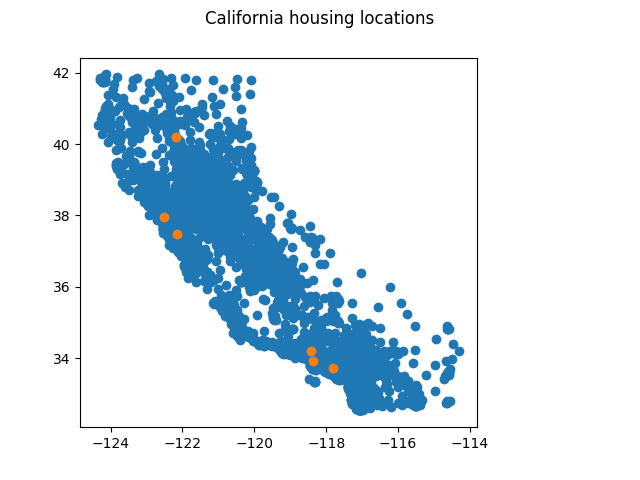
\includegraphics[width=\textwidth]{images/0.png}
		\caption{Initial }
		\label{figure:inital-nodes}
	\end{subfigure}\hfill
	\begin{subfigure}{0.5\columnwidth}
		\centering
		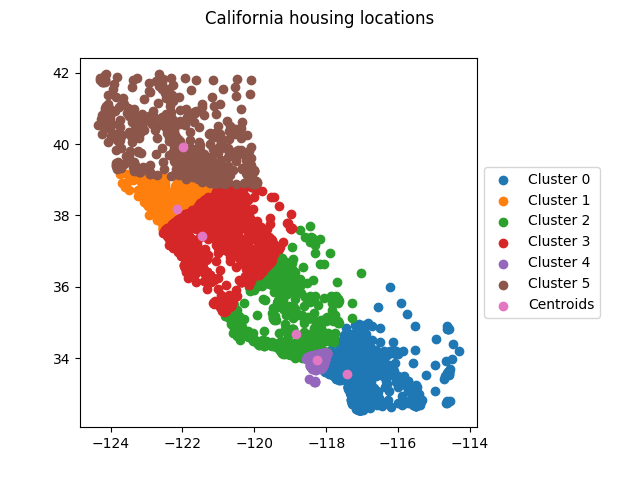
\includegraphics[width=\textwidth]{images/1.png}
		\caption{}
		\label{figure:iteration-1}
	\end{subfigure}
	
	\begin{subfigure}{0.5\columnwidth}
		\centering
		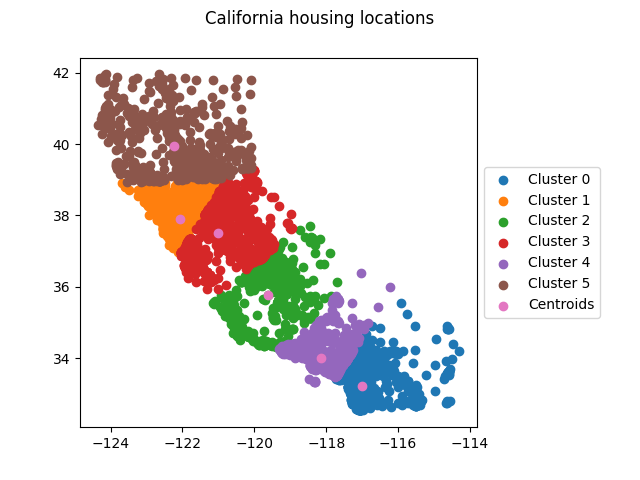
\includegraphics[width=\textwidth]{images/2.png}
		\caption{}
		\label{figure:iteration-2}
	\end{subfigure}\hfill
	\begin{subfigure}{0.5\columnwidth}
		\centering
		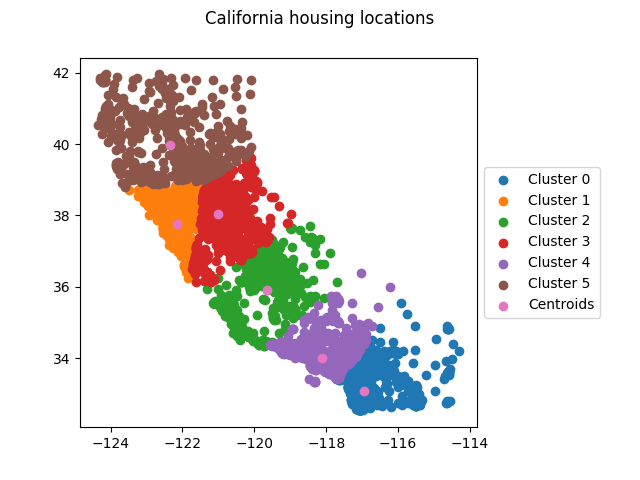
\includegraphics[width=\textwidth]{images/3.png}
		\caption{}
		\label{figure:iteration-3}
	\end{subfigure}
	
	\begin{subfigure}{0.5\columnwidth}
		\centering
		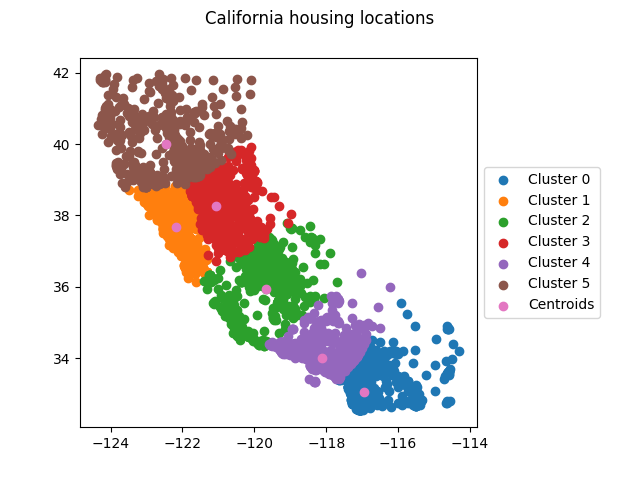
\includegraphics[width=\textwidth]{images/4.png}
		\caption{}
		\label{figure:iteration-4}
	\end{subfigure}\hfill
	\begin{subfigure}{0.5\columnwidth}
		\centering
		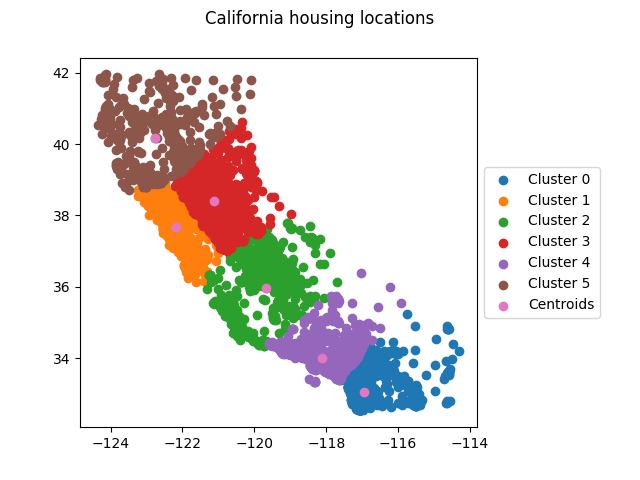
\includegraphics[width=\textwidth]{images/5.png}
		\caption{}
		\label{figure:iteration-5}
	\end{subfigure}
	
	\caption{K-Means algorithm used on housing locations from the \textit{California Housing Prices} dataset\cite{PJZZoRfZVMc9ZRlw}.}
	\label{figure:k-means-california-dataset}
\end{figure}
Looking at figure~\ref{figure:iteration-5}, it is interesting to note that the majority of centroids are in the vicinity of major cities in California, USA. For example, the centroid of Cluster 4 is near Los Angeles, the centroid for Cluster 2 is near Bakersfield, the centroid for Cluster 1 is near San Francisco, etc.




\section{Conclusion}\label{section:conclusion}
In summary, the K-Means algorithm was implemented in Python based on different sources\cite{Sharma19082019}\cite{IgcWaW8BViU6zM4T} for the purpose of this assignment project for the \textit{Statistical Pattern Recognition and Decision Making Methods} subject. The main objective of this work was to implement the method and use it on dataset. While the results overall seem to correlate with reality, there are discrepancies which the author was not able to remove or justify - perhaps more data (not just summary housing, but all housing) would be required for a more accurate result.



\nocite{Sharma19082019}
\bibliographystyle{IEEEtran}
\bibliography{references/references} 

\end{document}